% Beamer Presentation
% LaTeX Template
% Version 1.0 (10/11/12)
%
% This template has been downloaded from:
% http://www.LaTeXTemplates.com
%
% License:
% CC BY-NC-SA 3.0 (http://creativecommons.org/licenses/by-nc-sa/3.0/)
%
% Modified into a Beamer template for Northwestern University,
% by Daniel Lynch, 2019.
%
%%%%%%%%%%%%%%%%%%%%%%%%%%%%%%%%%%%%%%%%%

%----------------------------------------------------------------------------------------
%	PACKAGES AND THEMES
%----------------------------------------------------------------------------------------

\documentclass[aspectratio=169,9pt,xcolor=dvipsnames]{beamer}

\mode<presentation> {

% The Beamer class comes with a number of default slide themes
% which change the colors and layouts of slides. Below this is a list
% of all the themes, uncomment each in turn to see what they look like.

%\usetheme{default}
%\usetheme{AnnArbor}
%\usetheme{Antibes}
%\usetheme{Bergen}
\usetheme[hideothersubsections]{Berkeley}
%\usetheme{Berlin}
%\usetheme{Boadilla}
%\usetheme{CambridgeUS}
%\usetheme{Copenhagen}
%\usetheme{Darmstadt}
%\usetheme{Dresden}
%\usetheme{Frankfurt}
%\usetheme{Goettingen}
%\usetheme{Hannover}
%\usetheme{Ilmenau}
%\usetheme{JuanLesPins}
%\usetheme{Luebeck}
%\usetheme{Madrid}
%\usetheme{Malmoe}
%\usetheme{Marburg}
%\usetheme{Montpellier}
%\usetheme{PaloAlto}
%\usetheme{Pittsburgh}
%\usetheme{Rochester}
%\usetheme{Singapore}
%\usetheme{Szeged}
%\usetheme{Warsaw}

% As well as themes, the Beamer class has a number of color themes
% for any slide theme. Uncomment each of these in turn to see how it
% changes the colors of your current slide theme.

%\usecolortheme{albatross}
%\usecolortheme{beaver}
%\usecolortheme{beetle}
%\usecolortheme{crane}
%\usecolortheme{dolphin}
%\usecolortheme{dove}
%\usecolortheme{fly}
%\usecolortheme{lily}
%\usecolortheme{orchid}
%\usecolortheme{rose}
%\usecolortheme{seagull}
\usecolortheme{seahorse}
%\usecolortheme{whale}
%\usecolortheme{wolverine}

% Define NU color scheme:
% https://www.mccormick.northwestern.edu/marketing/logos-and-branding/color-usage-guidelines.html
\definecolor{NUpurple}{RGB}{078,042,132} % Northwestern Purple PMS 268, 0x4e2a84
\definecolor{purple60}{RGB}{131,110,170} % Purple 60, 0x836eaa
\definecolor{purple30}{RGB}{182,172,209} % Purple 30, 0xb6acd1
\definecolor{purple10}{RGB}{228,224,238} % Purple 10, 0xe4e0ee
\definecolor{purple120}{RGB}{064,031,104} % Purple 120, 0x401f68
\definecolor{black80}{HTML}{342F2E}     % Rich Black 80
\definecolor{black80}{HTML}{716C6B}     % Rich Black 50
\definecolor{black80}{HTML}{BBB8B8}     % Rich Black 20
\definecolor{black80}{HTML}{D8D6D6}     % Rich Black 10

\setbeamercolor{palette primary}{bg=NUpurple,fg=white}
\setbeamercolor{palette secondary}{bg=NUpurple,fg=white}
\setbeamercolor{palette tertiary}{bg=NUpurple,fg=white}
\setbeamercolor{palette quaternary}{bg=NUpurple,fg=white}
\setbeamercolor{structure}{fg=NUpurple} % itemize, enumerate, etc
\setbeamercolor{section in toc}{fg=NUpurple} % TOC sections

%\setbeamertemplate{footline} % To remove the footer line in all slides uncomment this line
\setbeamertemplate{footline}[page number] % To replace the footer line in all slides with a simple slide count uncomment this line

\setbeamertemplate{navigation symbols}{} % To remove the navigation symbols from the bottom of all slides uncomment this line
}

\usepackage{amsmath}
\usepackage{graphicx} % Allows including images
\usepackage{multimedia}
\usepackage{media9}
\usepackage{booktabs} % Allows the use of \toprule, \midrule and \bottomrule in tables
%\usepackage[orientation=landscape,size=custom,width=16,height=9,scale=0.5,debug]{beamerposter}
\usepackage{caption}
\captionsetup[figure]{labelformat=empty}% redefines the caption setup of the figures environment in the beamer class.
\usepackage{textpos}
\usepackage{tikz}
\usepackage{pgfpages}
\usepackage{listings}
\usepackage{multicol}

%----------------------------------------------------------------------------------------
% CUSTOM MACROS
%----------------------------------------------------------------------------------------
\newcommand{\etal}{et al. }
\newcommand{\ie}{i.e., }
\newcommand{\eg}{e.g., }

%----------------------------------------------------------------------------------------
%	TITLE PAGE
%----------------------------------------------------------------------------------------

\title[Intro]{A Short Guide to Destroying the Modern Information Marketplace} % The short title appears at the bottom of every slide, the full title is only on the title page

\author[Aerith Netzer]{Aerith Netzer} % Your name
\institute[NU] % Your institution as it will appear on the bottom of every slide, may be shorthand to save space
{
Digital Publishing and Repository Librarian \\ % Your institution for the title page
\medskip
Northwestern University Libraries \\ % Your institution for the title page
\medskip
\textit{aerith.netzer@northwestern.edu} % Your email address
}
\date{February 1, 2024} % Date, can be changed to a custom date

\begin{document}

\begin{frame}
\titlepage % Print the title page as the first slide
%\maketitle
%\vspace{-2.5cm}
%\includegraphics[width=\textwidth]{titleslide.eps}
\end{frame}

\addtobeamertemplate{frametitle}{}{
\begin{textblock*}{100mm}(.72\textwidth,-0.72cm)
\vspace{-0.1cm}

\includegraphics[width=4cm]{lockup-horizontal-short-white-rgb-eps-converted-to.pdf}
\end{textblock*}}

%----------------------------------------------------------------------------------------
%	PRESENTATION SLIDES
\section{Background}
\subsection{FOSS}
\begin{frame}
    \frametitle{FOSS Statement}
    \begin{block}{This Presentation's \LaTeX\ File is Available on GitHub}
        \begin{itemize}
            \item \url{https://www.github.com/aerithnetzer/OpenAI_Presentation}
        \end{itemize}
    \end{block}
    \begin{block}{The Code Demonstrated in this Presentation is Available on GitHub}
        \begin{itemize}
            \item \url{https://github.com/aerithnetzer/py-bats}
            \item \url{https://github.com/nulib-ds/publishing-template}
            \item \url{https://github.com/aerithnetzer/djournal}
        \end{itemize}
    \end{block}
\end{frame}
%------------------------------------------------
 % Sections can be created in order to organize your presentation into discrete blocks, all sections and subsections are automatically printed in the table of contents as an overview of the talk
%-----------------------------------------------
\subsection{Guerilla Open Access}
\begin{frame}
    \frametitle{Guiding Principles (Legally not instructions)}
\begin{quotation}
    Information is power. But like all power, there are those who want to keep it for themselves. The world’s entire scientific and cultural heritage, published over centuries in books and journals, is increasingly being digitized and locked up by a handful of private corporations. Want to read the papers featuring the most famous results of the sciences? You’ll need to send enormous amounts to publishers like Reed Elsevier.
(…)
We need to take information, wherever it is stored, make our copies and share them with the world. We need to take stuff that’s out of copyright and add it to the archive. We need to buy secret databases and put them on the Web. We need to download scientific journals and upload them to file sharing networks. We need to fight for Guerilla Open Access.
With enough of us, around the world, we’ll not just send a strong message opposing the privatization of knowledge — we’ll make it a thing of the past. Will you join us?
\end{quotation}
\begin{flushright}
    Aaron Swartz, 2008
    \\ \textit{Internet Archive, Guerilla Open Access Manifesto}
\end{flushright}
\end{frame}
\subsection{Vision}
\begin{frame}
    \frametitle{The Vision}
    \begin{center}
        \huge{Put the big publishers out of business.}
    \end{center}
    \begin{center}
        \small{Wiley, Elsevier, Springer, Taylor \& Francis, Sage, and others will not be able to compete with self-funded opertions like us.}
    \end{center}
\end{frame}

\subsection{Possibilities}
\begin{frame}
    \frametitle{This is Actually Possible!}
    \begin{center}
        \huge{\textit{Northwestern Insider} to be Published by Northwestern University Libraries!}
    \end{center}
    \begin{center}
        \large{Website created in two hours using Aerith's abstracted template of Chris Diaz's code.}
    \end{center}
\end{frame}

\subsection{O and A}
\begin{frame}{The Name of the Game}
    \begin{block}{Operationalize}
        \begin{itemize}
            \item Extend and abstract the current template created by Chris Diaz
            \item Host our own Open Journal Systems instance for future journals
            \item Create standard operating procedures for journal production and management
        \end{itemize}
    \end{block} % Add closing brace for "block" environment
    \begin{block}{Automate}
        \begin{itemize}
            \item Facilitate one-click (or few clicks) journal deployments
            \item Minimize reliance on outside vendors that we have to wait on to get things done
            \item Automate citation management, format construction, and metadata appending
        \end{itemize}
    \end{block} % Add closing brace for "block" environment
    
\end{frame}

\section*{JMSs}
\subsection{Challenges}
\begin{frame}
    \frametitle{Challenge: Journal Management Systems}
    \begin{center}
        \begin{block}{Challenges}
            \begin{itemize}
                \item OJS uses PHP
                \item OJS cannot be easily customized
                \item So archaic that almost no one hosts it themselves and relies on PKP
                \item Reliant on external vendors
            \end{itemize}
            
        \end{block}
    \end{center}
\end{frame}

\subsection{Solution}
\begin{frame}
    \frametitle{Solution: Djournal}
    \begin{center}
        \begin{block}{Djournal}
            \begin{itemize}
                \item A django application for journal management systems
                \item Homegrown
                \item Lightweight, elastic, and no more icky, icky PHP
            \end{itemize}
        \end{block}
    This is nowhere close to ready for deployment.
    \end{center}
    
\end{frame}


\section*{Website Design}
\subsection{Challenges}
\begin{frame}
    \frametitle{Challenges}
    \begin{center}
        \begin{tikzpicture}
            \node (markdown) at (0,0) {Markdown};
            \node (html) at (3,3) {HTML};
            \node (hugo) at (3,4) {Built with Hugo};
            \node (github) at (6,2) {Published Via GitHub Pages};

            \draw[->] (markdown) -- (html);
            \draw[-] (html) -- (hugo);
            \draw[-] (html) -- (github);
        \end{tikzpicture}
    \end{center}
    \begin{block}{Challenges}
        \begin{itemize}
            \item Have to create a new website for every journal
            \item Have to create edit the same HTML for every journal
            \item The current process is not scalable
        \end{itemize}
    \end{block}
\end{frame}
\subsection{Solutions}
\begin{frame}
    \frametitle{Templating Journal Websites}
    \begin{center}
    \url{https://github.com/nulib-ds/publishing-template}
    \begin{center}
        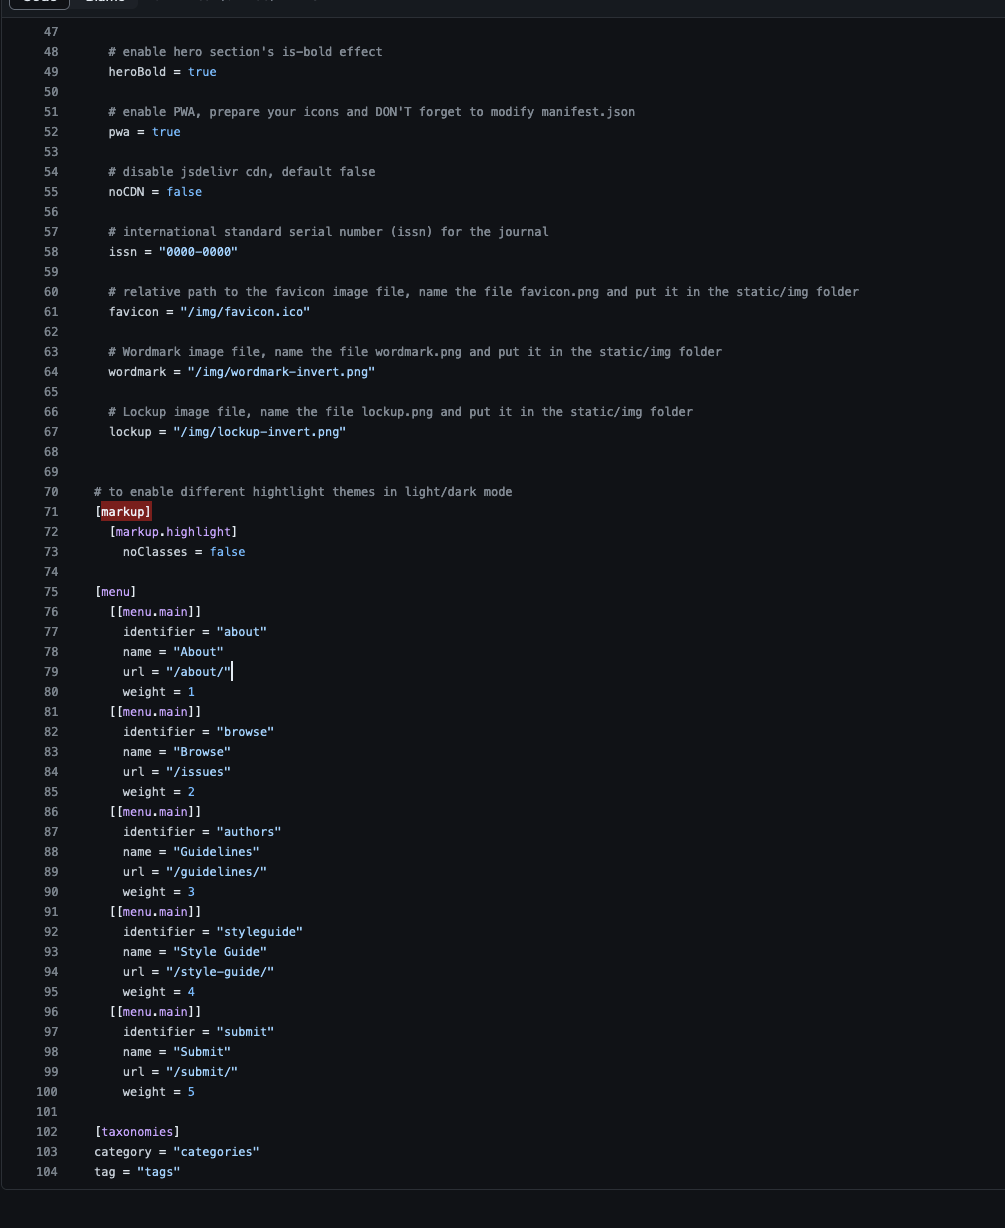
\includegraphics[width=\textwidth, height=\textheight, keepaspectratio]{config.png}
    \end{center}
    \end{center}
\end{frame}


\section{Citations}
\begin{frame}
    \frametitle{Challenges}
    \begin{center}
        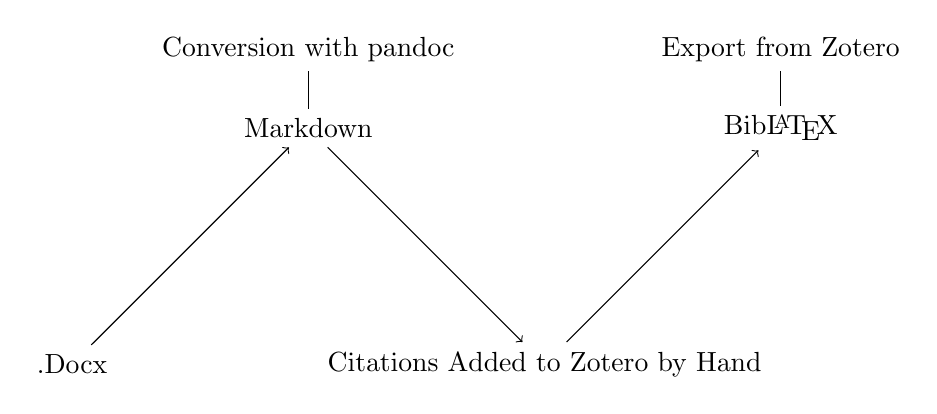
\begin{tikzpicture}
            \node (docx) at (0,0) {.Docx};
            \node (markdown) at (3,3) {Markdown};
            \node (zotero) at (6,0) {Citations Added to Zotero by Hand};
            \node (biblatex) at (9,3) {Bib\LaTeX};
            \node (pandoc) at (3,4) {Conversion with pandoc};
            \node (export) at (9,4) {Export from Zotero};
            
            \draw[->] (docx) -- (markdown);
            \draw[->] (markdown) -- (zotero);
            \draw[->] (zotero) -- (biblatex);
            \draw[-] (markdown) -- (pandoc);
            \draw[-] (biblatex) -- (export);
        \end{tikzpicture}
    \end{center}
        \begin{block}{The Current State is Not Scalable}
            \begin{itemize}
                \item The current process is time-consuming
                \item The current process is error-prone
                \item The current process is not scalable
                \item Reliant on inaccessible software
            \end{itemize}
        \end{block}
\end{frame}


%------------------------------------------------
\subsection{Problem \& Solution}
\begin{frame}[t]
    \frametitle{Solving Challenges}
    \begin{block}{The Problem of Plaintext Citations}
        \begin{itemize}
            \item Plaintext citations are not machine-readable
            \item Many different citation styles cause confusion
            \item Citations are often not linked to the cited work
        \end{itemize}
    \end{block}
    \begin{block}{Workaround: OpenAI GPT-3.5}
        \begin{itemize}
            \item Parse citations from article submission
            \item Create a .txt file with the citations in plaintext
            \item Call the OpenAI API to generate a Bib\LaTeX file
        \end{itemize}
    \end{block}
\begin{block}{The Optimal Solution: Bib\LaTeX\ Evangelising}
    \begin{itemize}
        \item Create resources that help create .bib files
        \item Communicate the importance of Bib\LaTeX\ to researchers
        \item Create a .tex file with the citations in Bib\LaTeX
    \end{itemize}
\end{block}
\centering
\end{frame}

%-------------------------------------------------
%Begin frame
\subsection{py-bats}
\begin{frame}{My Magnum Opus - py-bats}
    \begin{center}
        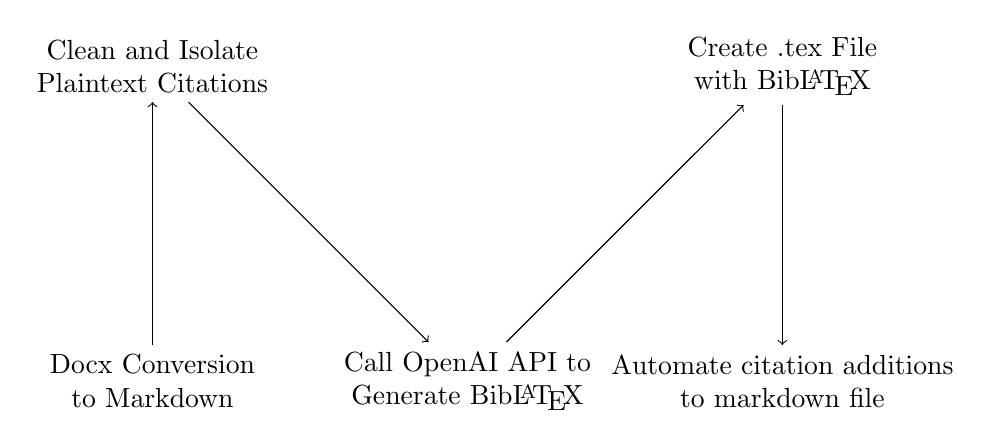
\begin{tikzpicture}
            \node[align=center] (data) at (-4,-2) {Docx Conversion \\ to Markdown};
            \node[align=center] (llm1) at (-4,2) {Clean and Isolate \\ Plaintext Citations};
            \node[align=center] (llm2) at (0,-2) {Call OpenAI API to \\ Generate Bib\LaTeX};
            \node[align=center] (llm3) at (4,2) {Create .tex File \\ with Bib\LaTeX};
            \node[align=center] (llm4) at (4, -2) {Automate citation additions \\ to markdown file};

            
            \draw[->] (data) -- (llm1);
            \draw[->] (llm1) -- (llm2);
            \draw[->] (llm2) -- (llm3);
            \draw[->] (llm3) -- (llm4);

        \end{tikzpicture}
    \end{center}
\end{frame}

%------------------------------------------------
\section{Future Work}
\subsection{The Roadmap}
\begin{frame}{The Roadmap}
    \begin{center}
        
\begin{tikzpicture}
            \node (data) at (0,0) {Data Creation};
            \node (llm1) at (5,0) {LLM Evaluation};
            \node (llm2) at (10,0) {LLM Fine-Tuning};
            
            \draw[->] (data) -- (llm1);
            \draw[->] (llm1) -- (llm2);
            
            \node [below] at (data.south) {Create a synthetic dataset};
            \node [below] at (llm1.south) {Out-of-the-box};
            \node [below] at (llm2.south) {Customized for citations};
        \end{tikzpicture}
    \end{center}
\end{frame}

%------------------------------------------------
\subsection{Journal Articles}
\begin{frame}{Output: Journal Article(s)}
    \begin{block}{Evaluating Large Language Models for Transforming Plaintext Citaitons to Machine-Readable Formats}
        \begin{itemize}
            \item Highlight the importance of Bib\LaTeX\ for citations and parsing by Google Scholar
            \item Create a synthetic dataset of plaintext citations and their Bib\LaTeX\ equivalents across many citation styles
            \item Evaluate the effectiveness and economic efficiency of large language models out-of-the-box
            \item Fine-tune a large language model to create a citation parser and measure its effectiveness and economic efficiency
        \end{itemize}
    \end{block}
    \begin{block}{A Modern, Maintainable, and Scalable Diamond Open Access Journal Publishing Workflow}
        \begin{itemize}
            \item Present hugo templating for journal websites
            \item Provide code, resources, and documentation for other libraries do spin up their own operations
        \end{itemize}
        
    \end{block}
\end{frame}

%------------------------------------------------
\subsection{Dev Work}
\begin{frame}{Development Opportunities}
    \begin{block}{Implementing Error Correction in Crossref API}
        \begin{itemize}
            \item Relatively often, HTML code is returned when Bib\LaTeX\ is requested
            \item Reduces effectiveness of the citation parser
            \item Error correction could be implemented to decrease confusion
        \end{itemize}
    \end{block}
\end{frame}
\section{Thanks!}
%------------------------------------------------------
\begin{frame}{A Quick Shoutout to People who contribute}
    \begin{block}{Chris Diaz}
        Because he should get some credit for building the website from which I made the template
    \end{block}
    \begin{block}{David Schober}
        For trusting me with access to GPT-3.5
    \end{block}
\end{frame}
%----------------------------------------------------------------------------------------
\begin{frame}{Finale}
    \centering
    Fin.
    
\end{frame}
\end{document} 
